% !TEX TS-program = pdflatex
\documentclass[11pt]{article}

% -------------------- Packages --------------------
\usepackage[a4paper,margin=1in]{geometry}
\usepackage{amsmath,amssymb}
\usepackage[T1]{fontenc}
\usepackage{lmodern}
\usepackage{xcolor}
\usepackage{tcolorbox}
\tcbuselibrary{skins,breakable}
\usepackage{enumitem}
\usepackage{hyperref}
\usepackage{tikz}
\usetikzlibrary{calc,angles,quotes,arrows.meta}

\pagestyle{empty}

% -------------------- Dark Theme Colors --------------------
\definecolor{bg}{HTML}{000000}
\definecolor{pairbg}{HTML}{121212}
\definecolor{solbg}{HTML}{0A0A0A}
\definecolor{border}{HTML}{2A2A2A}
\definecolor{text}{HTML}{FFFFFF}
\definecolor{muted}{HTML}{C9CDD3}
\definecolor{gold}{HTML}{FFD700}
\definecolor{green}{HTML}{4ADE80}
\definecolor{cyan}{HTML}{38BDF8}

\pagecolor{bg}
\color{text}

\hypersetup{
  colorlinks=true,
  linkcolor=cyan,
  urlcolor=cyan
}

\setlength{\parindent}{0pt}
\setlength{\parskip}{10pt}

% Help LaTeX avoid overfull lines globally
\sloppy
\setlength{\emergencystretch}{3em}

\setlist[itemize]{left=1.4em,itemsep=6pt,topsep=6pt}
\setlist[enumerate]{left=1.6em,itemsep=4pt,topsep=4pt}

% -------------------- tcolorbox Base --------------------
\tcbset{
  enhanced,
  breakable,
  arc=12pt,
  boxrule=0.8pt,
  left=14pt,right=14pt,top=12pt,bottom=12pt
}

\newtcolorbox{QAPair}[1]{%
  colback=pairbg,
  colbacklower=solbg,
  colframe=border,
  coltext=text,
  title=\textcolor{gold}{\bfseries #1},
  fonttitle=\bfseries,
  coltitle=text,
  segmentation style={draw=border, dashed, line width=0.6pt},
  before upper=\raggedright,
  before lower=\raggedright
}

\newtcolorbox{QuickBox}{%
  colback=pairbg,
  colframe=cyan,
  coltext=text,
  fontupper=\color{text}\raggedright,
  borderline north={4pt}{0pt}{cyan},
  arc=14pt,
  boxrule=0.8pt
}

% Helper for step headings
\newcommand{\Step}[1]{\textcolor{muted}{\textbf{Step #1:}}}

% Small centered diagram block
\newenvironment{StepDiagram}{\par\medskip\begin{center}}{\end{center}\medskip}

% TikZ styles
\tikzset{
  base/.style={draw=text, line width=0.9pt, line cap=round, line join=round},
  new/.style={draw=cyan, line width=1.2pt, line cap=round, line join=round},
  help/.style={draw=muted, dashed, line width=0.9pt},
  ang/.style={draw=gold, line width=1.0pt},
  dot/.style={circle, fill=text, inner sep=1.2pt},
  lab/.style={text=text, font=\small},
  labm/.style={text=muted, font=\small},
  labfill/.style={lab, fill=pairbg, inner sep=1.2pt},
}

\newcommand{\EqDiagram}[1]{%
\begin{StepDiagram}
\begin{tikzpicture}
\node[draw=border, rounded corners=10pt, inner sep=8pt, text=text, align=left, text width=0.86\linewidth] {#1};
\end{tikzpicture}
\end{StepDiagram}
}

% ============================================================
\begin{document}

\begin{center}
{\LARGE\bfseries \textcolor{gold}{Exercise 10.1 --- Solutions}}\\[-2pt]
\end{center}

% -------------------- Quick formulas (each line has its own diagram) --------------------
\begin{QuickBox}
{\color{cyan}\bfseries Quick formulas (Tangents \& angles of a circle)}\par\medskip
\begin{itemize}

\item \textbf{Radius $\perp$ tangent:} If $PT$ is tangent at $T$ and $O$ is centre, then $OT\perp PT$.
\begin{StepDiagram}
\begin{tikzpicture}[scale=0.95]
  \def\r{1.8}
  \coordinate (O) at (0,0);
  \coordinate (T) at (\r,0);
  \coordinate (U) at (\r,1.6);
  \coordinate (V) at (\r,-1.6);
  \coordinate (P) at (\r,1.15);

  \draw[base] (O) circle (\r);
  \node[dot,label={[lab]below:$O$}] at (O) {};
  \node[dot,label={[lab]right:$T$}] at (T) {};
  \node[dot,label={[lab]right:$P$}] at (P) {};

  \draw[new] (O)--(T);
  \draw[new] (U)--(V); % tangent
  \node[labm] at ($(U)+(0.55,0)$) {tangent $PT$};

  % right angle mark at T between OT and tangent
  \draw[base] ($(T)+(-0.18,0)$) -- ($(T)+(-0.18,0.18)$) -- ($(T)+(0,0.18)$);

  \node[labm] at (0,-2.25) {$OT\perp$ tangent at $T$};
\end{tikzpicture}
\end{StepDiagram}

\item \textbf{Equal tangents:} From an external point $A$, tangents $AB$ and $AC$ satisfy $AB=AC$.
\begin{StepDiagram}
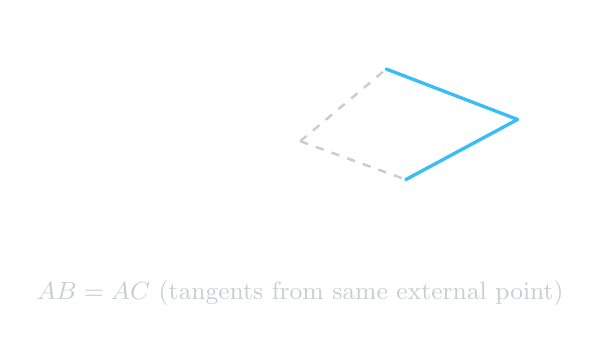
\begin{tikzpicture}[scale=0.92]
  \def\r{1.55}
  \coordinate (O) at (0,0);
  \coordinate (A) at (3.0,0.3);

  % Choose tangency points (approx)
  \coordinate (B) at ({\r*cos(40)},{\r*sin(40)});
  \coordinate (C) at ({\r*cos(-20)},{\r*sin(-20)});

  \draw[base] (O) circle (\r);
  \node[dot,label={[lab]below:$O$}] at (O) {};
  \node[dot,label={[lab]right:$A$}] at (A) {};
  \node[dot,label={[lab]above right:$B$}] at (B) {};
  \node[dot,label={[lab]below right:$C$}] at (C) {};

  \draw[new] (A)--(B);
  \draw[new] (A)--(C);
  \draw[help] (O)--(B);
  \draw[help] (O)--(C);

  % right angle marks at B and C
  \draw[base] ($(B)+(-0.12,-0.02)$) -- ($(B)+(-0.12,0.16)$) -- ($(B)+(0.04,0.16)$);
  \draw[base] ($(C)+(-0.12,0.02)$) -- ($(C)+(-0.12,-0.16)$) -- ($(C)+(0.04,-0.16)$);

  \node[labm] at (0,-2.10) {$AB=AC$ (tangents from same external point)};
\end{tikzpicture}
\end{StepDiagram}

\item \textbf{Power of a point:} If from $A$, $AB$ is a tangent and $A$--$D$ is a secant meeting the circle at $E$ and $D$, then
\[
AB^2=AE\cdot AD.
\]
\begin{StepDiagram}
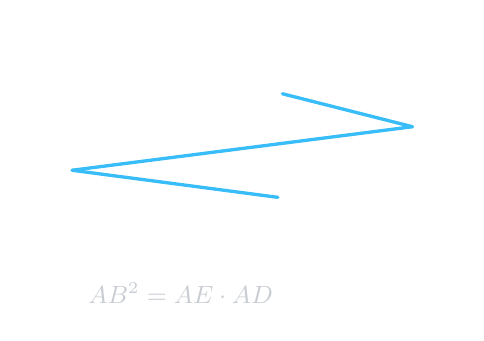
\begin{tikzpicture}[scale=0.92]
  \def\r{1.55}
  \coordinate (O) at (0,0);
  \coordinate (A) at (3.2,0.2);
  \coordinate (B) at ({\r*cos(25)},{\r*sin(25)});
  \coordinate (E) at ({\r*cos(195)},{\r*sin(195)});
  \coordinate (D) at ({\r*cos(330)},{\r*sin(330)});

  \draw[base] (O) circle (\r);
  \node[dot,label={[lab]below:$O$}] at (O) {};
  \node[dot,label={[lab]right:$A$}] at (A) {};
  \node[dot,label={[lab]above:$B$}] at (B) {};
  \node[dot,label={[lab]left:$E$}] at (E) {};
  \node[dot,label={[lab]below:$D$}] at (D) {};

  % tangent AB at B (not perfect, but schematic)
  \draw[new] (A)--(B);

  % secant A-E-D
  \draw[new] (A)--(E);
  \draw[new] (E)--(D);

  \node[labm] at (0,-2.10) {$AB^2=AE\cdot AD$};
\end{tikzpicture}
\end{StepDiagram}

\item \textbf{Tangent--chord theorem:} Angle between a tangent and a chord equals the angle in the opposite segment.
\begin{StepDiagram}
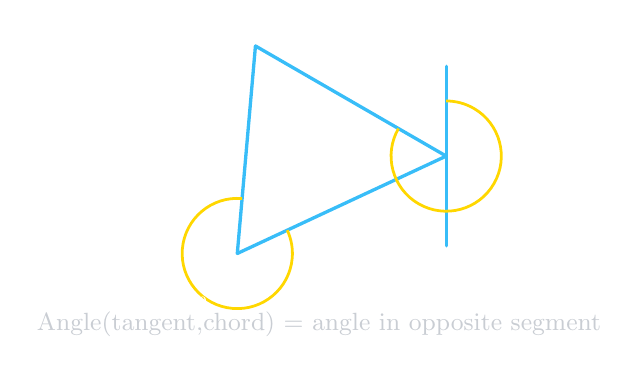
\begin{tikzpicture}[scale=0.95]
  \def\r{1.7}
  \coordinate (O) at (0,0);
  \coordinate (T) at (\r,0);
  \coordinate (A) at ({\r*cos(120)},{\r*sin(120)});
  \coordinate (B) at ({\r*cos(230)},{\r*sin(230)});
  \coordinate (P) at (\r,1.2);
  \coordinate (Q) at (\r,-1.2);

  \draw[base] (O) circle (\r);
  \node[dot,label={[lab]below:$O$}] at (O) {};
  \node[dot,label={[lab]right:$T$}] at (T) {};
  \node[dot,label={[lab]left:$A$}] at (A) {};
  \node[dot,label={[lab]below left:$B$}] at (B) {};

  % tangent at T
  \draw[new] (P)--(Q);

  % chord TA and inscribed angle at B
  \draw[new] (T)--(A);
  \draw[new] (B)--(A);
  \draw[new] (B)--(T);

  \pic[ang,"$\theta$",lab,angle radius=7mm,angle eccentricity=1.25] {angle=A--T--P};
  \pic[ang,"$\theta$",lab,angle radius=7mm,angle eccentricity=1.15] {angle=A--B--T};

  \node[labm] at (0,-2.25) {Angle(tangent,chord) = angle in opposite segment};
\end{tikzpicture}
\end{StepDiagram}

\item \textbf{Angle between two tangents:} If tangents from $A$ touch at $B$ and $C$, then
\[
\angle BAC = 180^\circ-\angle BOC.
\]
\begin{StepDiagram}
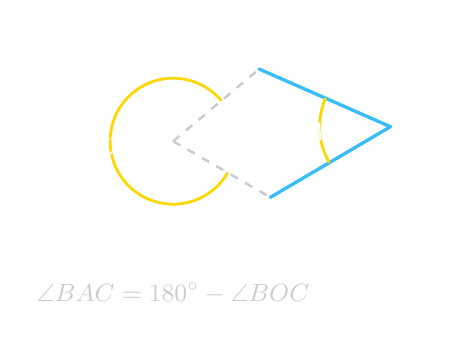
\begin{tikzpicture}[scale=0.92]
  \def\r{1.55}
  \coordinate (O) at (0,0);
  \coordinate (A) at (3.0,0.2);
  \coordinate (B) at ({\r*cos(40)},{\r*sin(40)});
  \coordinate (C) at ({\r*cos(-30)},{\r*sin(-30)});

  \draw[base] (O) circle (\r);
  \node[dot,label={[lab]below:$O$}] at (O) {};
  \node[dot,label={[lab]right:$A$}] at (A) {};
  \node[dot,label={[lab]above right:$B$}] at (B) {};
  \node[dot,label={[lab]below right:$C$}] at (C) {};

  \draw[new] (A)--(B);
  \draw[new] (A)--(C);
  \draw[help] (O)--(B);
  \draw[help] (O)--(C);

  \pic[ang,"$\angle BAC$",lab,angle radius=9mm,angle eccentricity=1.2] {angle=B--A--C};
  \pic[ang,"$\angle BOC$",lab,angle radius=8mm,angle eccentricity=1.2] {angle=B--O--C};

  \node[labm] at (0,-2.10) {$\angle BAC = 180^\circ-\angle BOC$};
\end{tikzpicture}
\end{StepDiagram}

\end{itemize}
\end{QuickBox}

% ============================================================
% Q1(i)
\begin{QAPair}{Question 1 (i)}
\textcolor{gold}{\bfseries Question:} In the figure, $PQ$ is tangent to the circle at $Q$, $OP=13$ cm and $PQ=12$ cm. Find $r=OQ$.
\tcblower
\textcolor{green}{\bfseries Answer:}\par

\Step{1} Since $PQ$ is tangent at $Q$, $OQ\perp PQ$. So $\triangle OPQ$ is right-angled at $Q$.
\begin{StepDiagram}
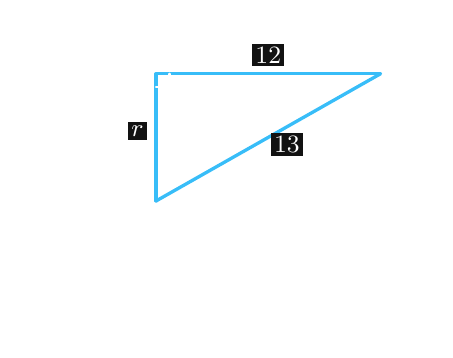
\begin{tikzpicture}[scale=0.95]
  \def\r{1.7}
  \coordinate (O) at (0,0);
  \coordinate (Q) at (0,\r);
  \coordinate (P) at (3.0,\r);

  \draw[base] (O) circle (\r);
  \node[dot,label={[lab]left:$O$}] at (O) {};
  \node[dot,label={[lab]above:$Q$}] at (Q) {};
  \node[dot,label={[lab]right:$P$}] at (P) {};

  \draw[new] (O)--(Q);
  \draw[new] (Q)--(P);
  \draw[new] (O)--(P);

  \draw[base] ($(Q)+(0,-0.18)$) -- ($(Q)+(0.18,-0.18)$) -- ($(Q)+(0.18,0)$);

  \node[labfill] at ($(Q)!0.5!(P)+(0,0.25)$) {$12$};
  \node[labfill] at ($(O)!0.55!(P)+(0.10,-0.18)$) {$13$};
  \node[labfill] at ($(O)!0.55!(Q)+(-0.25,0)$) {$r$};
\end{tikzpicture}
\end{StepDiagram}

\Step{2} By Pythagoras:
\[
OP^2=OQ^2+PQ^2
\Rightarrow 13^2=r^2+12^2
\Rightarrow r^2=25
\Rightarrow r=5\text{ cm}.
\]
\EqDiagram{$13^2=r^2+12^2 \Rightarrow r^2=169-144=25 \Rightarrow r=5$}

\[
\boxed{r=5\text{ cm}}
\]
\end{QAPair}

% ============================================================
% Q1(ii)
\begin{QAPair}{Question 1 (ii)}
\textcolor{gold}{\bfseries Question:} Radius $OM=2$ cm and tangent segment $ML=6\sqrt3$ cm. Find $d=OL$.
\tcblower
\textcolor{green}{\bfseries Answer:}\par

\Step{1} $OM\perp ML$ (radius to tangent point), so $\triangle OML$ is right-angled at $M$.
\begin{StepDiagram}
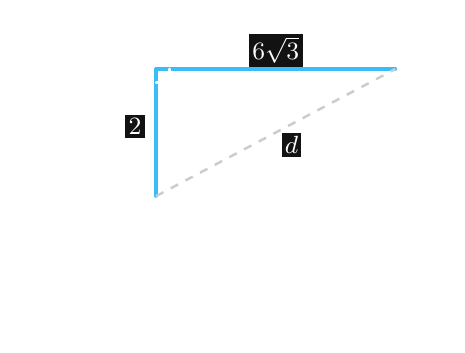
\begin{tikzpicture}[scale=0.95]
  \coordinate (O) at (0,0);
  \coordinate (M) at (0,1.7);
  \coordinate (L) at (3.2,1.7);

  \draw[base] (O) circle (1.7);
  \node[dot,label={[lab]left:$O$}] at (O) {};
  \node[dot,label={[lab]above:$M$}] at (M) {};
  \node[dot,label={[lab]right:$L$}] at (L) {};

  \draw[new] (O)--(M);
  \draw[new] (M)--(L);
  \draw[help] (O)--(L);

  \draw[base] ($(M)+(0,-0.18)$) -- ($(M)+(0.18,-0.18)$) -- ($(M)+(0.18,0)$);

  \node[labfill] at ($(O)!0.55!(M)+(-0.28,0)$) {$2$};
  \node[labfill] at ($(M)!0.5!(L)+(0,0.25)$) {$6\sqrt3$};
  \node[labfill] at ($(O)!0.55!(L)+(0.05,-0.25)$) {$d$};
\end{tikzpicture}
\end{StepDiagram}
\EqDiagram{$OL^2=OM^2+ML^2$}

\Step{2} Compute:
\[
d^2=2^2+(6\sqrt3)^2=4+108=112
\Rightarrow d=\sqrt{112}=4\sqrt7\text{ cm}.
\]
\EqDiagram{$d=\sqrt{112}=4\sqrt7$}

\[
\boxed{d=4\sqrt7\text{ cm}}
\]
\end{QAPair}

% ============================================================
% Q1(iii)
\begin{QAPair}{Question 1 (iii)}
\textcolor{gold}{\bfseries Question:} From external point $A$, $AB$ and $AC$ are tangents. Given $AB=8$ cm and $\angle BAP=30^\circ$ (where $P$ is centre). Find $x=AC$ and $y=PB$.
\tcblower
\textcolor{green}{\bfseries Answer:}\par

\Step{1} Tangents from the same external point are equal:
\[
AC=AB=8 \Rightarrow x=8\text{ cm}.
\]
\begin{StepDiagram}
\begin{tikzpicture}[scale=0.92]
  \def\r{1.55}
  \coordinate (P) at (0,0);
  \coordinate (A) at (3.1,0.2);
  \coordinate (B) at ({\r*cos(35)},{\r*sin(35)});
  \coordinate (C) at ({\r*cos(-25)},{\r*sin(-25)});

  \draw[base] (P) circle (\r);
  \node[dot,label={[lab]below:$P$}] at (P) {};
  \node[dot,label={[lab]right:$A$}] at (A) {};
  \node[dot,label={[lab]above right:$B$}] at (B) {};
  \node[dot,label={[lab]below right:$C$}] at (C) {};

  \draw[new] (A)--(B);
  \draw[new] (A)--(C);
  \node[labm] at (0,-2.05) {$AB=AC$};
\end{tikzpicture}
\end{StepDiagram}

\Step{2} In $\triangle PAB$, $PB\perp AB$ (radius to tangent point). With $\angle BAP=30^\circ$,
\[
\tan 30^\circ=\frac{PB}{AB}\Rightarrow PB=AB\tan 30^\circ
=8\cdot\frac{1}{\sqrt3}=\frac{8\sqrt3}{3}.
\]
\begin{StepDiagram}
\begin{tikzpicture}[scale=0.92]
  \def\r{1.55}
  \coordinate (P) at (0,0);
  \coordinate (B) at (0,\r);
  \coordinate (A) at (3.0,\r);

  \draw[base] (P) circle (\r);
  \node[dot,label={[lab]below:$P$}] at (P) {};
  \node[dot,label={[lab]above:$B$}] at (B) {};
  \node[dot,label={[lab]right:$A$}] at (A) {};

  \draw[new] (A)--(B); % tangent
  \draw[new] (P)--(B); % radius
  \draw[help] (P)--(A);

  \draw[base] ($(B)+(0,-0.18)$) -- ($(B)+(0.18,-0.18)$) -- ($(B)+(0.18,0)$);

  \pic[ang,"$30^\circ$",lab,angle radius=8mm,angle eccentricity=1.2] {angle=B--A--P};

  \node[labfill] at ($(A)!0.5!(B)+(0,0.25)$) {$8$};
  \node[labfill] at ($(P)!0.55!(B)+(-0.28,0)$) {$y$};
\end{tikzpicture}
\end{StepDiagram}
\EqDiagram{$PB=8\tan 30^\circ=\dfrac{8}{\sqrt3}=\dfrac{8\sqrt3}{3}$}

\[
\boxed{x=8\text{ cm}\qquad y=\frac{8\sqrt3}{3}\text{ cm}}
\]
\end{QAPair}

% ============================================================
% Q1(iv)
\begin{QAPair}{Question 1 (iv)}
\textcolor{gold}{\bfseries Question:} From $A$, $AB$ and $AC$ are tangents and $\angle BAC=25^\circ$. If $x=\angle OBC$ and $y=\angle OCB$, find $x$ and $y$.
\tcblower
\textcolor{green}{\bfseries Answer:}\par

\Step{1} Angle between tangents and the central angle:
\[
\angle BAC=180^\circ-\angle BOC
\Rightarrow \angle BOC=180^\circ-25^\circ=155^\circ.
\]
\begin{StepDiagram}
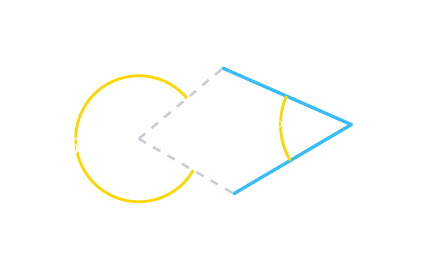
\begin{tikzpicture}[scale=0.90]
  \def\r{1.55}
  \coordinate (O) at (0,0);
  \coordinate (A) at (3.0,0.2);
  \coordinate (B) at ({\r*cos(40)},{\r*sin(40)});
  \coordinate (C) at ({\r*cos(-30)},{\r*sin(-30)});

  \draw[base] (O) circle (\r);
  \node[dot,label={[lab]below:$O$}] at (O) {};
  \node[dot,label={[lab]right:$A$}] at (A) {};
  \node[dot,label={[lab]above right:$B$}] at (B) {};
  \node[dot,label={[lab]below right:$C$}] at (C) {};

  \draw[new] (A)--(B);
  \draw[new] (A)--(C);
  \draw[help] (O)--(B);
  \draw[help] (O)--(C);

  \pic[ang,"$25^\circ$",lab,angle radius=9mm,angle eccentricity=1.2] {angle=B--A--C};
  \pic[ang,"$155^\circ$",lab,angle radius=8mm,angle eccentricity=1.15] {angle=B--O--C};
\end{tikzpicture}
\end{StepDiagram}
\EqDiagram{$\angle BOC=155^\circ$}

\Step{2} In $\triangle OBC$, $OB=OC$ (radii), so base angles are equal:
\[
x=y=\frac{180^\circ-155^\circ}{2}=12.5^\circ=12^\circ30'.
\]
\begin{StepDiagram}
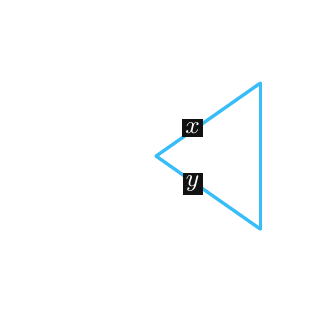
\begin{tikzpicture}[scale=0.95]
  \def\r{1.7}
  \coordinate (O) at (0,0);
  \coordinate (B) at ({\r*cos(35)},{\r*sin(35)});
  \coordinate (C) at ({\r*cos(-35)},{\r*sin(-35)});

  \draw[base] (O) circle (\r);
  \node[dot,label={[lab]below:$O$}] at (O) {};
  \node[dot,label={[lab]above right:$B$}] at (B) {};
  \node[dot,label={[lab]below right:$C$}] at (C) {};

  \draw[new] (O)--(B);
  \draw[new] (O)--(C);
  \draw[new] (B)--(C);

  \node[labfill] at ($(B)!0.72!(O)+(0.10,0.10)$) {$x$};
  \node[labfill] at ($(C)!0.72!(O)+(0.10,-0.10)$) {$y$};
\end{tikzpicture}
\end{StepDiagram}
\EqDiagram{$x=y=12.5^\circ$}

\[
\boxed{x=y=12.5^\circ\;(=12^\circ30')}
\]
\end{QAPair}

% ============================================================
% Q1(v)
\begin{QAPair}{Question 1 (v)}
\textcolor{gold}{\bfseries Question:} In the figure, $AB$ is tangent with $AB=15$ cm. The centre is $C$ and $\angle DBC=30^\circ$. Find $a=\angle BAC$ and the external segment $b$.
\tcblower
\textcolor{green}{\bfseries Answer:}\par

\Step{1} Since $CB=CD$ (radii), $\triangle BCD$ is isosceles. Given $\angle DBC=30^\circ$, so $\angle BDC=30^\circ$ and
\[
\angle BCD=180^\circ-30^\circ-30^\circ=120^\circ.
\]
\begin{StepDiagram}
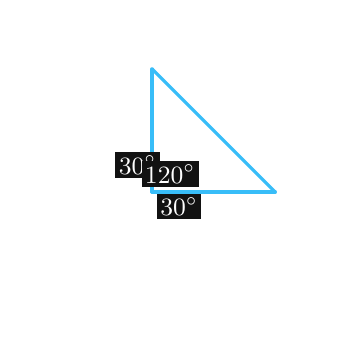
\begin{tikzpicture}[scale=0.92]
  \def\r{1.7}
  \coordinate (C) at (0,0);
  \coordinate (B) at (0,\r);
  \coordinate (D) at (\r,0);

  \draw[base] (C) circle (\r);
  \node[dot,label={[lab]below:$C$}] at (C) {};
  \node[dot,label={[lab]above:$B$}] at (B) {};
  \node[dot,label={[lab]right:$D$}] at (D) {};

  \draw[new] (C)--(B);
  \draw[new] (C)--(D);
  \draw[new] (B)--(D);

  \node[labfill] at ($(B)!0.78!(C)+(-0.20,0)$) {$30^\circ$};
  \node[labfill] at ($(D)!0.78!(C)+(0,-0.20)$) {$30^\circ$};
  \node[labfill] at ($(C)+(0.25,0.25)$) {$120^\circ$};
\end{tikzpicture}
\end{StepDiagram}

\Step{2} $A,C,D$ are collinear, so
\[
\angle BCA = 180^\circ-\angle BCD=180^\circ-120^\circ=60^\circ.
\]
\begin{StepDiagram}
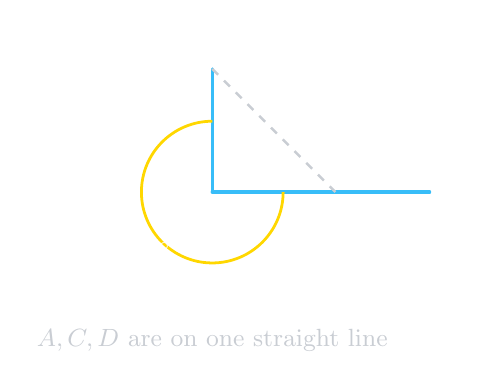
\begin{tikzpicture}[scale=0.92]
  \def\r{1.7}
  \coordinate (C) at (0,0);
  \coordinate (B) at (0,\r);
  \coordinate (D) at (\r,0);
  \coordinate (A) at (3.0,0);

  \draw[base] (C) circle (\r);
  \node[dot,label={[lab]below:$C$}] at (C) {};
  \node[dot,label={[lab]above:$B$}] at (B) {};
  \node[dot,label={[lab]right:$D$}] at (D) {};
  \node[dot,label={[lab]right:$A$}] at (A) {};

  \draw[new] (C)--(B);
  \draw[new] (C)--(A);
  \draw[help] (B)--(D);

  \pic[ang,"$60^\circ$",lab,angle radius=9mm,angle eccentricity=1.2] {angle=B--C--A};
  \node[labm] at (0,-2.05) {$A,C,D$ are on one straight line};
\end{tikzpicture}
\end{StepDiagram}
\EqDiagram{$\angle BCA=60^\circ$}

\Step{3} In $\triangle ABC$, $CB\perp AB$ (radius to tangent), hence $\angle ABC=90^\circ$.
Therefore,
\[
a=\angle BAC=180^\circ-90^\circ-60^\circ=30^\circ.
\]
\begin{StepDiagram}
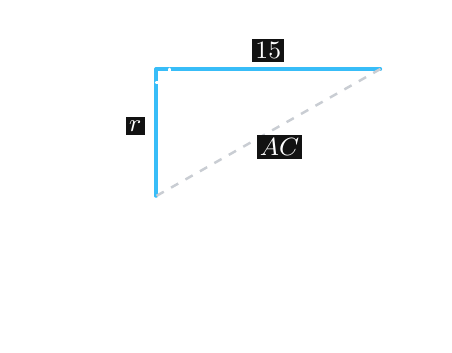
\begin{tikzpicture}[scale=0.95]
  \coordinate (C) at (0,0);
  \coordinate (B) at (0,1.7);
  \coordinate (A) at (3.0,1.7);

  \draw[base] (C) circle (1.7);
  \node[dot,label={[lab]below:$C$}] at (C) {};
  \node[dot,label={[lab]above:$B$}] at (B) {};
  \node[dot,label={[lab]right:$A$}] at (A) {};

  \draw[new] (A)--(B); % tangent
  \draw[new] (C)--(B); % radius
  \draw[help] (A)--(C);

  \draw[base] ($(B)+(0,-0.18)$) -- ($(B)+(0.18,-0.18)$) -- ($(B)+(0.18,0)$);

  \node[labfill] at ($(A)!0.5!(B)+(0,0.25)$) {$15$};
  \node[labfill] at ($(C)!0.55!(B)+(-0.28,0)$) {$r$};
  \node[labfill] at ($(C)!0.55!(A)+(0,-0.28)$) {$AC$};
\end{tikzpicture}
\end{StepDiagram}
\EqDiagram{$a=30^\circ$}

\Step{4} Use right triangle $\triangle ABC$:
\[
\cos a=\frac{AB}{AC}
\Rightarrow \cos 30^\circ=\frac{15}{AC}
\Rightarrow AC=10\sqrt3.
\]
Also,
\[
CB=AC\sin 30^\circ = 5\sqrt3.
\]
External segment:
\[
b=AC-CB = 10\sqrt3-5\sqrt3=5\sqrt3.
\]
\EqDiagram{$AC=10\sqrt3,\;\;CB=5\sqrt3,\;\;b=AC-CB=5\sqrt3$}

\[
\boxed{a=30^\circ\qquad b=5\sqrt3\text{ cm}}
\]
\end{QAPair}

% ============================================================
% Q1(vi)
\begin{QAPair}{Question 1 (vi)}
\textcolor{gold}{\bfseries Question:} From $A$, $AB$ and $AC$ are tangents. Given $\angle BPC=120^\circ$ (centre $P$). Find $a=\angle BAC$ and $b=\angle PCD$.
\tcblower
\textcolor{green}{\bfseries Answer:}\par

\Step{1} Angle between tangents:
\[
a=\angle BAC=180^\circ-\angle BPC=180^\circ-120^\circ=60^\circ.
\]
\begin{StepDiagram}
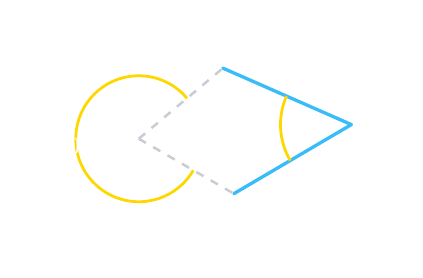
\begin{tikzpicture}[scale=0.90]
  \def\r{1.55}
  \coordinate (P) at (0,0);
  \coordinate (A) at (3.0,0.2);
  \coordinate (B) at ({\r*cos(40)},{\r*sin(40)});
  \coordinate (C) at ({\r*cos(-30)},{\r*sin(-30)});

  \draw[base] (P) circle (\r);
  \node[dot,label={[lab]below:$P$}] at (P) {};
  \node[dot,label={[lab]right:$A$}] at (A) {};
  \node[dot,label={[lab]above right:$B$}] at (B) {};
  \node[dot,label={[lab]below right:$C$}] at (C) {};

  \draw[new] (A)--(B);
  \draw[new] (A)--(C);
  \draw[help] (P)--(B);
  \draw[help] (P)--(C);

  \pic[ang,"$120^\circ$",lab,angle radius=8mm,angle eccentricity=1.15] {angle=B--P--C};
  \pic[ang,"$a$",lab,angle radius=9mm,angle eccentricity=1.2] {angle=B--A--C};
\end{tikzpicture}
\end{StepDiagram}
\EqDiagram{$a=60^\circ$}

\Step{2} From the figure, $B,P,D$ are collinear (so $BD$ is a diameter line). Hence
\[
\angle CPD = 180^\circ-\angle CPB = 180^\circ-120^\circ=60^\circ.
\]
In $\triangle PCD$, $PC=PD$ (radii), so base angles are equal:
\[
b=\angle PCD=\frac{180^\circ-60^\circ}{2}=60^\circ.
\]
\begin{StepDiagram}
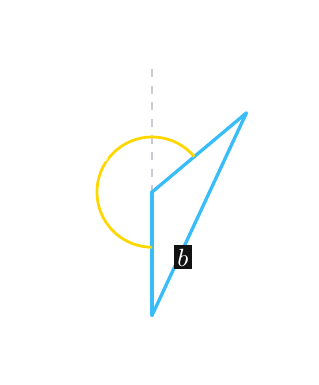
\begin{tikzpicture}[scale=0.92]
  \def\r{1.7}
  \coordinate (P) at (0,0);
  \coordinate (B) at (0,\r);
  \coordinate (D) at (0,-\r);
  \coordinate (C) at ({\r*cos(40)},{\r*sin(40)});

  \draw[base] (P) circle (\r);
  \node[dot,label={[lab]right:$P$}] at (P) {};
  \node[dot,label={[lab]above:$B$}] at (B) {};
  \node[dot,label={[lab]below:$D$}] at (D) {};
  \node[dot,label={[lab]right:$C$}] at (C) {};

  \draw[help] (B)--(D);
  \draw[new] (P)--(C);
  \draw[new] (P)--(D);
  \draw[new] (C)--(D);

  \node[labfill] at ($(C)!0.75!(D)+(0.10,0.10)$) {$b$};
  \pic[ang,"$60^\circ$",lab,angle radius=7mm,angle eccentricity=1.2] {angle=C--P--D};
\end{tikzpicture}
\end{StepDiagram}
\EqDiagram{$b=60^\circ$}

\[
\boxed{a=60^\circ\qquad b=60^\circ}
\]
\end{QAPair}

% ============================================================
% Q1(vii)
\begin{QAPair}{Question 1 (vii)}
\textcolor{gold}{\bfseries Question:} In the figure, the tangent at $A$ makes $75^\circ$ with chord $AB$ and $\angle DAB=90^\circ$. Find $\alpha=\angle ABD$.
\tcblower
\textcolor{green}{\bfseries Answer:}\par

\Step{1} By the tangent--chord theorem, the angle between tangent at $A$ and chord $AB$ equals the angle in the opposite segment:
\[
\angle ADB = 75^\circ.
\]
\begin{StepDiagram}
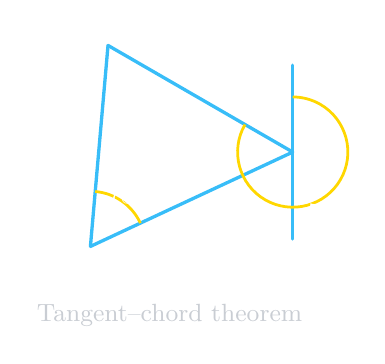
\begin{tikzpicture}[scale=0.92]
  \def\r{1.7}
  \coordinate (O) at (0,0);
  \coordinate (A) at (\r,0);
  \coordinate (B) at ({\r*cos(120)},{\r*sin(120)});
  \coordinate (D) at ({\r*cos(230)},{\r*sin(230)});
  \coordinate (P) at (\r,1.2);
  \coordinate (Q) at (\r,-1.2);

  \draw[base] (O) circle (\r);
  \node[dot,label={[lab]right:$A$}] at (A) {};
  \node[dot,label={[lab]left:$B$}] at (B) {};
  \node[dot,label={[lab]below left:$D$}] at (D) {};

  \draw[new] (P)--(Q);   % tangent at A
  \draw[new] (A)--(B);   % chord AB
  \draw[new] (A)--(D);   % chord AD
  \draw[new] (B)--(D);   % chord BD

  \pic[ang,"$75^\circ$",lab,angle radius=7mm,angle eccentricity=1.25] {angle=B--A--P};
  \pic[ang,"$75^\circ$",lab,angle radius=7mm,angle eccentricity=1.15] {angle=A--D--B};

  \node[labm] at (0,-2.25) {Tangent--chord theorem};
\end{tikzpicture}
\end{StepDiagram}
\EqDiagram{So, $\angle ADB=75^\circ$}

\Step{2} In $\triangle ABD$:
\[
\alpha=\angle ABD = 180^\circ-\angle DAB-\angle ADB
=180^\circ-90^\circ-75^\circ=15^\circ.
\]
\EqDiagram{$\alpha=15^\circ$}

\[
\boxed{\alpha=15^\circ}
\]
\end{QAPair}

% ============================================================
% Q1(viii)
\begin{QAPair}{Question 1 (viii)}
\textcolor{gold}{\bfseries Question:} At $A$, a tangent touches the circle. The angles between the tangent and chords are $63^\circ$ (with $AB$) and $57^\circ$ (with $AC$). Find $x=\angle ACB$, $y=\angle BAC$, and $z=\angle ABC$.
\tcblower
\textcolor{green}{\bfseries Answer:}\par

\Step{1} Tangent--chord theorem for chord $AB$:
\[
x=\angle ACB = 63^\circ.
\]
\begin{StepDiagram}
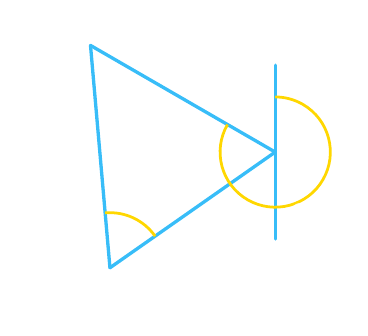
\begin{tikzpicture}[scale=0.92]
  \def\r{1.7}
  \coordinate (O) at (0,0);
  \coordinate (A) at (\r,0);
  \coordinate (B) at ({\r*cos(120)},{\r*sin(120)});
  \coordinate (C) at ({\r*cos(250)},{\r*sin(250)});
  \coordinate (P) at (\r,1.2);
  \coordinate (Q) at (\r,-1.2);

  \draw[base] (O) circle (\r);
  \node[dot,label={[lab]right:$A$}] at (A) {};
  \node[dot,label={[lab]left:$B$}] at (B) {};
  \node[dot,label={[lab]below left:$C$}] at (C) {};

  \draw[new] (P)--(Q);  % tangent at A
  \draw[new] (A)--(B);
  \draw[new] (A)--(C);
  \draw[new] (B)--(C);

  \pic[ang,"$63^\circ$",lab,angle radius=7mm,angle eccentricity=1.25] {angle=B--A--P};
  \pic[ang,"$x$",lab,angle radius=7mm,angle eccentricity=1.15] {angle=A--C--B};
\end{tikzpicture}
\end{StepDiagram}
\EqDiagram{$x=63^\circ$}

\Step{2} Tangent--chord theorem for chord $AC$:
\[
z=\angle ABC = 57^\circ.
\]
\begin{StepDiagram}
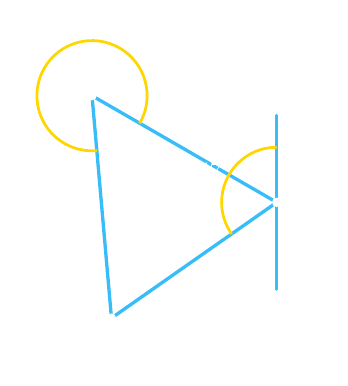
\begin{tikzpicture}[scale=0.92]
  \def\r{1.7}
  \coordinate (O) at (0,0);
  \coordinate (A) at (\r,0);
  \coordinate (B) at ({\r*cos(120)},{\r*sin(120)});
  \coordinate (C) at ({\r*cos(250)},{\r*sin(250)});
  \coordinate (P) at (\r,1.2);
  \coordinate (Q) at (\r,-1.2);

  \draw[base] (O) circle (\r);
  \draw[new] (P)--(Q);  % tangent
  \draw[new] (A)--(B);
  \draw[new] (A)--(C);
  \draw[new] (B)--(C);

  \node[dot,label={[lab]right:$A$}] at (A) {};
  \node[dot,label={[lab]left:$B$}] at (B) {};
  \node[dot,label={[lab]below left:$C$}] at (C) {};

  \pic[ang,"$57^\circ$",lab,angle radius=7mm,angle eccentricity=1.25] {angle=P--A--C};
  \pic[ang,"$z$",lab,angle radius=7mm,angle eccentricity=1.15] {angle=A--B--C};
\end{tikzpicture}
\end{StepDiagram}
\EqDiagram{$z=57^\circ$}

\Step{3} Use triangle angle sum:
\[
y=180^\circ-x-z=180^\circ-63^\circ-57^\circ=60^\circ.
\]
\EqDiagram{$y=60^\circ$}

\[
\boxed{x=63^\circ\qquad y=60^\circ\qquad z=57^\circ}
\]
\end{QAPair}

% ============================================================
% Q2
\begin{QAPair}{Question 2}
\textcolor{gold}{\bfseries Question:} $AB$ and $AC$ are tangents to a circle with centre $O$ at $B$ and $C$.
If $\angle BOC=120^\circ$, find:
(i) $\angle OBA$ \quad (ii) $\angle OCB$ \quad (iii) $\angle BAC$ \quad (iv) $\angle ABC$.
\tcblower
\textcolor{green}{\bfseries Answer:}\par

\Step{1} Radius to tangent point is perpendicular:
\[
\angle OBA=90^\circ,\qquad \angle OCB=90^\circ.
\]
\begin{StepDiagram}
\begin{tikzpicture}[scale=0.90]
  \def\r{1.6}
  \coordinate (O) at (0,0);
  \coordinate (B) at ({\r*cos(50)},{\r*sin(50)});
  \coordinate (C) at ({\r*cos(-70)},{\r*sin(-70)});
  \coordinate (A) at (3.0,0.2);

  \draw[base] (O) circle (\r);
  \node[dot,label={[lab]below:$O$}] at (O) {};
  \node[dot,label={[lab]above right:$B$}] at (B) {};
  \node[dot,label={[lab]below right:$C$}] at (C) {};
  \node[dot,label={[lab]right:$A$}] at (A) {};

  \draw[new] (A)--(B);
  \draw[new] (A)--(C);
  \draw[new] (O)--(B);
  \draw[new] (O)--(C);

  \draw[base] ($(B)+(-0.10,-0.02)$) -- ($(B)+(-0.10,0.14)$) -- ($(B)+(0.04,0.14)$);
  \draw[base] ($(C)+(-0.10,0.02)$) -- ($(C)+(-0.10,-0.14)$) -- ($(C)+(0.04,-0.14)$);
\end{tikzpicture}
\end{StepDiagram}

\Step{2} Angle between tangents:
\[
\angle BAC=180^\circ-\angle BOC=180^\circ-120^\circ=60^\circ.
\]
\begin{StepDiagram}
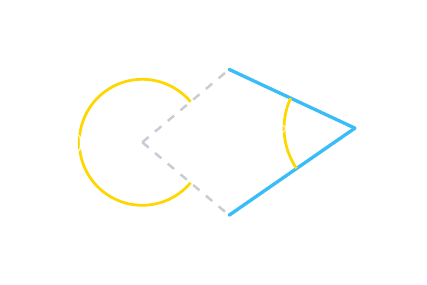
\begin{tikzpicture}[scale=0.90]
  \def\r{1.6}
  \coordinate (O) at (0,0);
  \coordinate (A) at (3.0,0.2);
  \coordinate (B) at ({\r*cos(40)},{\r*sin(40)});
  \coordinate (C) at ({\r*cos(-40)},{\r*sin(-40)});

  \draw[base] (O) circle (\r);
  \node[dot,label={[lab]below:$O$}] at (O) {};
  \node[dot,label={[lab]right:$A$}] at (A) {};
  \node[dot,label={[lab]above right:$B$}] at (B) {};
  \node[dot,label={[lab]below right:$C$}] at (C) {};

  \draw[new] (A)--(B);
  \draw[new] (A)--(C);
  \draw[help] (O)--(B);
  \draw[help] (O)--(C);

  \pic[ang,"$120^\circ$",lab,angle radius=8mm,angle eccentricity=1.15] {angle=B--O--C};
  \pic[ang,"$60^\circ$",lab,angle radius=9mm,angle eccentricity=1.2] {angle=B--A--C};
\end{tikzpicture}
\end{StepDiagram}

\Step{3} Since $AB=AC$ (tangents from $A$), $\triangle ABC$ is isosceles, so
\[
\angle ABC=\angle ACB=\frac{180^\circ-60^\circ}{2}=60^\circ.
\]
\EqDiagram{$\angle ABC=60^\circ$}

\[
\boxed{\angle OBA=90^\circ,\;\angle OCB=90^\circ,\;\angle BAC=60^\circ,\;\angle ABC=60^\circ}
\]
\end{QAPair}

% ============================================================
% Q3
\begin{QAPair}{Question 3}
\textcolor{gold}{\bfseries Question:} $O$ is the centre of two concentric circles. $AB$ and $CD$ are chords of the outer circle tangent to the inner circle. Prove that $AB=CD$.
\tcblower
\textcolor{green}{\bfseries Answer:}\par

\Step{1} If chord $AB$ is tangent to the inner circle, then the perpendicular distance from $O$ to chord $AB$ equals the inner radius (say $r$). Similarly, distance from $O$ to chord $CD$ is also $r$.
\begin{StepDiagram}
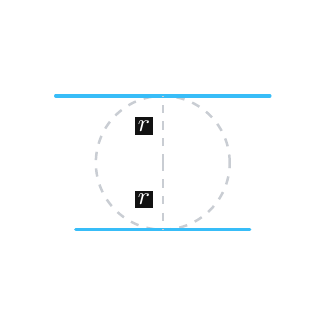
\begin{tikzpicture}[scale=0.85]
  \def\R{2.0}
  \def\r{1.0}
  \coordinate (O) at (0,0);

  \draw[base] (O) circle (\R);
  \draw[help] (O) circle (\r);
  \node[dot,label={[lab]below:$O$}] at (O) {};

  % chord AB tangent to inner circle at top
  \coordinate (A) at (-1.6,1.0);
  \coordinate (B) at ( 1.6,1.0);
  \draw[new] (A)--(B);

  % chord CD tangent to inner circle at bottom
  \coordinate (C) at (-1.3,-1.0);
  \coordinate (D) at ( 1.3,-1.0);
  \draw[new] (C)--(D);

  % perpendiculars
  \coordinate (M) at (0,1.0);
  \coordinate (N) at (0,-1.0);
  \draw[help] (O)--(M);
  \draw[help] (O)--(N);

  \node[labfill] at ($(O)!0.55!(M)+(-0.28,0)$) {$r$};
  \node[labfill] at ($(O)!0.55!(N)+(-0.28,0)$) {$r$};
\end{tikzpicture}
\end{StepDiagram}

\Step{2} In the \emph{same outer circle}, chords that are equidistant from the centre are equal in length.
\EqDiagram{Same circle + equal distances from centre $\Rightarrow$ equal chords}

\Step{3} Since $\text{dist}(O,AB)=\text{dist}(O,CD)=r$, we conclude
\[
AB=CD.
\]
\EqDiagram{$AB=CD$}

\[
\boxed{AB=CD}
\]
\end{QAPair}

% ============================================================
% Q4
\begin{QAPair}{Question 4}
\textcolor{gold}{\bfseries Question:} Ali whirls a stone with a string of length $3$ ft. The string breaks and the stone moves along the tangent and hits a point $5$ ft away from Ali. Find the distance covered by the stone.
\tcblower
\textcolor{green}{\bfseries Answer:}\par

\Step{1} Ali is the centre. Radius to the stone at the break point is $3$ ft, and the stone moves along the tangent, which is perpendicular to the radius.
\begin{StepDiagram}
\begin{tikzpicture}[scale=0.95]
  \def\r{1.6}
  \coordinate (A) at (0,0); % Ali
  \coordinate (S) at (\r,0); % stone at break
  \coordinate (H) at (\r,1.8); % hit point direction (tangent)
  \draw[base] (A) circle (\r);

  \node[dot,label={[lab]below:Ali}] at (A) {};
  \node[dot,label={[lab]right:$S$}] at (S) {};
  \node[dot,label={[lab]right:Hit}] at (H) {};

  \draw[new] (A)--(S);
  \draw[new] (S)--(H);
  \draw[base] ($(S)+(-0.18,0)$) -- ($(S)+(-0.18,0.18)$) -- ($(S)+(0,0.18)$);

  \node[labfill] at ($(A)!0.55!(S)+(0,-0.25)$) {$3$};
\end{tikzpicture}
\end{StepDiagram}

\Step{2} Form a right triangle with hypotenuse $5$ ft (Ali to hit point) and one leg $3$ ft (radius). If $s$ is the distance travelled:
\[
3^2+s^2=5^2 \Rightarrow s^2=16 \Rightarrow s=4\text{ ft}.
\]
\EqDiagram{$s=\sqrt{5^2-3^2}=\sqrt{16}=4$}

\[
\boxed{4\text{ ft}}
\]
\end{QAPair}

% ============================================================
% Q5
\begin{QAPair}{Question 5}
\textcolor{gold}{\bfseries Question:} Three circles touch externally. The ratio of distances between their centres is $2:3:4$.
The perimeter of the triangle formed by joining the centres is $36$ cm. Find the radius of each circle.
\tcblower
\textcolor{green}{\bfseries Answer:}\par

\Step{1} Let the side lengths (distances between centres) be $2k,3k,4k$.
\[
2k+3k+4k=9k=36 \Rightarrow k=4.
\]
So the distances are $8,12,16$ cm.
\EqDiagram{$k=4 \Rightarrow (2k,3k,4k)=(8,12,16)$}
\begin{StepDiagram}
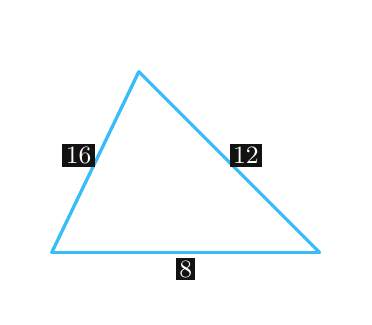
\begin{tikzpicture}[scale=0.85]
  \coordinate (A) at (0,0);
  \coordinate (B) at (4.0,0);
  \coordinate (C) at (1.3,2.7);

  \node[dot,label={[lab]below:$C_1$}] at (A) {};
  \node[dot,label={[lab]below:$C_2$}] at (B) {};
  \node[dot,label={[lab]above:$C_3$}] at (C) {};

  \draw[new] (A)--(B);
  \draw[new] (B)--(C);
  \draw[new] (C)--(A);

  \node[labfill] at ($(A)!0.5!(B)+(0,-0.25)$) {$8$};
  \node[labfill] at ($(B)!0.5!(C)+(0.25,0.10)$) {$12$};
  \node[labfill] at ($(C)!0.5!(A)+(-0.25,0.10)$) {$16$};
\end{tikzpicture}
\end{StepDiagram}

\Step{2} If the radii are $r_1,r_2,r_3$ and the circles touch externally, then each distance equals a sum of two radii:
\[
r_1+r_2=8,\quad r_2+r_3=12,\quad r_3+r_1=16.
\]
\EqDiagram{External touch: centre distance $=$ sum of radii}

\Step{3} Add all:
\[
2(r_1+r_2+r_3)=36 \Rightarrow r_1+r_2+r_3=18.
\]
Solve:
\[
r_1=6,\quad r_2=2,\quad r_3=10.
\]
\EqDiagram{$r_1=6,\;r_2=2,\;r_3=10$}

\[
\boxed{r_1=6\text{ cm},\; r_2=2\text{ cm},\; r_3=10\text{ cm}}
\]
\end{QAPair}

% ============================================================
% Q6
\begin{QAPair}{Question 6}
\textcolor{gold}{\bfseries Question:} In the figure, $AD=5$ cm, $CD=4$ cm and $BD=4.5$ cm. Find the distance between the centres of the circles.
\tcblower
\textcolor{green}{\bfseries Answer:}\par

\Step{1} The line through $C$ is a common tangent at $C$, hence $AC\perp CD$ and $BC\perp CD$.
So $\triangle ACD$ and $\triangle BCD$ are right-angled at $C$.
\begin{StepDiagram}
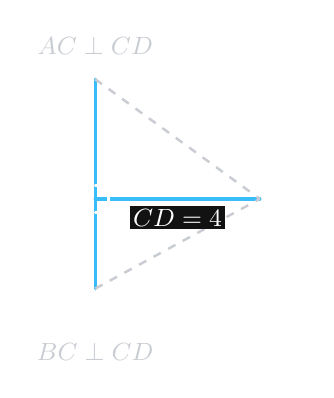
\begin{tikzpicture}[scale=0.95]
  \coordinate (C) at (0,0);
  \coordinate (D) at (2.2,0); % along tangent
  \coordinate (A) at (0,1.6);
  \coordinate (B) at (0,-1.2);

  \node[dot,label={[lab]below:$C$}] at (C) {};
  \node[dot,label={[lab]right:$D$}] at (D) {};
  \node[dot,label={[lab]left:$A$}] at (A) {};
  \node[dot,label={[lab]left:$B$}] at (B) {};

  \draw[new] (C)--(D); % tangent segment
  \draw[new] (A)--(C);
  \draw[new] (B)--(C);
  \draw[help] (A)--(D);
  \draw[help] (B)--(D);

  \draw[base] ($(C)+(0,0.18)$) -- ($(C)+(0.18,0.18)$) -- ($(C)+(0.18,0)$);
  \draw[base] ($(C)+(0,-0.18)$) -- ($(C)+(0.18,-0.18)$) -- ($(C)+(0.18,0)$);

  \node[labfill] at ($(C)!0.5!(D)+(0,-0.25)$) {$CD=4$};
  \node[labm] at (0,2.05) {$AC\perp CD$};
  \node[labm] at (0,-2.05) {$BC\perp CD$};
\end{tikzpicture}
\end{StepDiagram}

\Step{2} Use Pythagoras to find radii:
\[
AC=\sqrt{AD^2-CD^2}=\sqrt{5^2-4^2}=3,
\quad
BC=\sqrt{BD^2-CD^2}=\sqrt{4.5^2-4^2}=\frac{\sqrt{17}}{2}.
\]
\EqDiagram{$AC=3,\;\;BC=\dfrac{\sqrt{17}}{2}$}

\Step{3} Since the circles touch externally at $C$, the distance between centres is
\[
AB=AC+BC=3+\frac{\sqrt{17}}{2}=\frac{6+\sqrt{17}}{2}\text{ cm}.
\]
\EqDiagram{$AB=3+\dfrac{\sqrt{17}}{2}$}

\[
\boxed{AB=\frac{6+\sqrt{17}}{2}\text{ cm}\;\approx 5.06\text{ cm}}
\]
\end{QAPair}

% ============================================================
% Q7
\begin{QAPair}{Question 7}
\textcolor{gold}{\bfseries Question:} In the adjoining figure, $\angle PEF=20^\circ$. $H$ is the midpoint of $FG$. Find $\angle PGH$.
\tcblower
\textcolor{green}{\bfseries Answer:}\par

\Step{1} $EF$ is tangent at $F$, so $PF\perp EF$. Thus $\triangle PEF$ is right-angled at $F$.
\[
\angle EPF=180^\circ-90^\circ-20^\circ=70^\circ.
\]
\begin{StepDiagram}
\begin{tikzpicture}[scale=0.90]
  \def\r{1.6}
  \coordinate (P) at (0,0);
  \coordinate (F) at (\r,0);
  \coordinate (E) at (\r,1.9);

  \draw[base] (P) circle (\r);
  \node[dot,label={[lab]below:$P$}] at (P) {};
  \node[dot,label={[lab]right:$F$}] at (F) {};
  \node[dot,label={[lab]right:$E$}] at (E) {};

  \draw[new] (P)--(F);
  \draw[new] (F)--(E); % tangent segment
  \draw[base] ($(F)+(-0.18,0)$) -- ($(F)+(-0.18,0.18)$) -- ($(F)+(0,0.18)$);

  \pic[ang,"$20^\circ$",lab,angle radius=7mm,angle eccentricity=1.2] {angle=P--E--F};
\end{tikzpicture}
\end{StepDiagram}
\EqDiagram{$\angle EPF=70^\circ$}

\Step{2} Points $E,P,G$ are collinear, so
\[
\angle GPF = 180^\circ-\angle EPF=180^\circ-70^\circ=110^\circ.
\]
\EqDiagram{$\angle GPF=110^\circ$}

\Step{3} In $\triangle PFG$, $PF=PG$ (radii), so base angles are equal:
\[
\angle PGF=\angle PFG=\frac{180^\circ-110^\circ}{2}=35^\circ.
\]
\begin{StepDiagram}
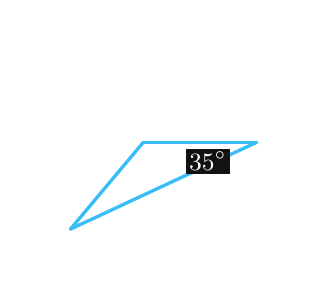
\begin{tikzpicture}[scale=0.90]
  \def\r{1.6}
  \coordinate (P) at (0,0);
  \coordinate (F) at (\r,0);
  \coordinate (G) at ({\r*cos(230)},{\r*sin(230)});
  \coordinate (E) at (2.2,0); % collinear with P and G direction (schematic)

  \draw[base] (P) circle (\r);
  \node[dot,label={[lab]below:$P$}] at (P) {};
  \node[dot,label={[lab]right:$F$}] at (F) {};
  \node[dot,label={[lab]below left:$G$}] at (G) {};

  \draw[new] (P)--(F);
  \draw[new] (P)--(G);
  \draw[new] (F)--(G);

  \node[labfill] at ($(G)!0.70!(F)+(0.10,0.10)$) {$35^\circ$};
\end{tikzpicture}
\end{StepDiagram}
\EqDiagram{$\angle PGF=35^\circ$}

\Step{4} Since $H$ lies on chord $FG$, ray $GH$ is the same direction as $GF$, hence
\[
\angle PGH=\angle PGF=35^\circ.
\]
\EqDiagram{$\angle PGH=35^\circ$}

\[
\boxed{\angle PGH=35^\circ}
\]
\end{QAPair}

% ============================================================
% Q8
\begin{QAPair}{Question 8}
\textcolor{gold}{\bfseries Question:} In the figure, $AB=AC$ (tangents from $A$). Given angle between tangent at $B$ and chord $BD$ is $46^\circ$, and $\angle BDC=66^\circ$. Find $x=\angle BAC$ and $y$ (angle between tangent at $C$ and chord $CD$).
\tcblower
\textcolor{green}{\bfseries Answer:}\par

\Step{1} By tangent--chord theorem at $B$ (tangent with chord $BD$),
\[
\angle BCD = 46^\circ.
\]
\begin{StepDiagram}
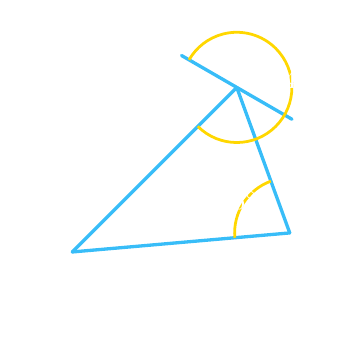
\begin{tikzpicture}[scale=0.90]
  \def\r{1.7}
  \coordinate (O) at (0,0);
  \coordinate (B) at ({\r*cos(60)},{\r*sin(60)});
  \coordinate (C) at ({\r*cos(-20)},{\r*sin(-20)});
  \coordinate (D) at ({\r*cos(210)},{\r*sin(210)});
  \coordinate (Tb1) at ($(B)+( {-0.9*sin(60)} , {0.9*cos(60)} )$);
  \coordinate (Tb2) at ($(B)+( { 0.9*sin(60)} , {-0.9*cos(60)} )$);

  \draw[base] (O) circle (\r);
  \node[dot,label={[lab]below:$O$}] at (O) {};
  \node[dot,label={[lab]above:$B$}] at (B) {};
  \node[dot,label={[lab]right:$C$}] at (C) {};
  \node[dot,label={[lab]below left:$D$}] at (D) {};

  \draw[new] (D)--(B);
  \draw[new] (D)--(C);
  \draw[new] (B)--(C);

  \draw[new] (Tb1)--(Tb2); % tangent at B (schematic)

  \pic[ang,"$46^\circ$",lab,angle radius=7mm,angle eccentricity=1.2] {angle=D--B--Tb1};
  \pic[ang,"$46^\circ$",lab,angle radius=7mm,angle eccentricity=1.1] {angle=B--C--D};
\end{tikzpicture}
\end{StepDiagram}
\EqDiagram{$\angle BCD=46^\circ$}

\Step{2} In $\triangle BCD$:
\[
\angle DBC = 180^\circ-66^\circ-46^\circ=68^\circ.
\]
\EqDiagram{$\angle DBC=68^\circ$}

\Step{3} By tangent--chord theorem at $C$ (tangent with chord $CD$),
\[
y=\angle(\text{tangent at }C,\; CD)=\angle DBC=68^\circ.
\]
\EqDiagram{$y=68^\circ$}

\Step{4} Central angle on chord $BC$:
\[
\angle BOC = 2\angle BDC = 2\cdot 66^\circ=132^\circ.
\]
Angle between tangents:
\[
x=\angle BAC = 180^\circ-\angle BOC = 48^\circ.
\]
\EqDiagram{$x=48^\circ$}

\[
\boxed{x=48^\circ\qquad y=68^\circ}
\]
\end{QAPair}

\end{document}
